\section{Introduction}
    \label{s:intro}
    The number of analysis tools required in multidisciplinary design optimization (MDO) studies is growing
    in parallel with the increasing scope of typical MDO problems. An example of this growth in scope can
    be observed in the historical evolution of the disciplines involved in MDO problems in aircraft design.
    Multidisciplinary optimization emerged as a separate field from structural optimization through the
    need to introduce formal techniques for managing the coupling of aerodynamic loads and structural
    deformations, through the linking of aerodynamic vortex lattice or panel methods with structural finite
    element models [[REF]]. Subsequently, flight performance and life cycle economics tools were integrated
    into MDO analysis workflows for conceptual and preliminary design studies [[REF]]. Currently, MDO
    problems for aircraft design also often include tools for aircraft noise and emissions. In sum, it is now
    commonplace for 5-10 analysis tools to be employed for typical aircraft design optimization studies [[REF]].
    
    The number of analysis tools is expected to grow in the future as the scope of MDO problems continues
    to evolve, and as computing is increasingly commoditized. This expansion of scope will be driven, in
    part, by consideration of additional disciplines. Current trends on the horizon for aircraft MDO studies
    include incorporation of manufacturing analyses [[REF]], subsystem performance [[REF]], and fleet-level
    aggregate models of emissions, noise, or economics [[REF]].

    As the size and complexity of engineering systems grow, the time and expense for setting up 
    analysis models grow with them. Multidisciplinary Design Analysis and Optimization (MDAO)
    frameworks such as OpenMDAO\cite{Gray2012} and ModelCenter have enabled a new level of analysis tool integration 
    and paved the way for models with more analyses and increasing numbers of interdisciplinary couplings. That 
    new capability has created a new challenge. Even for models with 10's of analyses there could be hundreds or thousands
    of variables that need to be linked together. Commonly different analyses will provide competing values for the 
    same physical quantity, and these conflicts need to be resolved somehow. To make matters worse, the competeing values 
    may not even be in the same format. These occurrences are particularly acute when analysis tools have differing fidelities. For
    example, an abstracted aerodynamic analysis such as an empirical drag buildup model may return only
    integrated drag, whereas a CFD tool may return pressure and shear stress distributions across the entire
    surface grid. If an analysis downstream of the aerodynamics tool needs only integrated drag as an input,
    then the designer has a free choice of which of the two possible aerodynamics analysis tools to select to
    provide the drag estimate (presuming that drag can be computed from surface distributions by a simple
    integration algorithm). On the other hand, if a downstream analysis needs a pressure distribution in
    order to compute pitching moment, for example, then any feasible MDO problem formulation must
    include CFD or similar analysis in the data flow, regardless of whether the empirical drag buildup model
    is also included.

    With all the added complexity from larger models it is not hard to imagine that the task of combining all the analyses into a 
    consistent system model capable of solving a relevant engineering design 
    problem could easily become much more costly than createing the discipline 
    analyses themselves. Just as for a large system the couplings between the 
    disciplines begin to dominate the design space, the couplings between the 
    analyses begin to dominate the job of setting up the model. It is this problem of 
    determining sets of analysis tools and their interconnectivities to form realistic
    multidisciplinary problems that is the subject of this paper. We are motivated by the following notional
    but real problem of organizing an MDO study for a complex system:

    A new system is being designed for which there is little or no historical precedent. The system
    is complex, as measured by the number of disciplines and/or components involved in the
    analysis. A general optimization problem statement has been formulated based on system-
    level objectives and constraints; however, it is unclear which engineering analysis tools should
    be interconnected in order to solve the optimization problem. A team of disciplinary and/
    or component design engineers has been formed in which each engineer has expertise in a
    particular analysis tool or component model. The engineers meet to discuss the approach to
    interconnecting their tools to achieve the required system-level MDO model.
    
    Our goal is to develop formalism for expressing analysis interconnectivity and for determining feasible
    data flows to assist an engineering team conducting this task. Because the problem deals with
    interconnectivity, we base our approach on the representations and techniques of graph theory. The 
    proposed graph syntax is closely related to the REMS system proposed by 
    Alexandrov and Lewis\cite{alexandrov2004}. The approach taken here should be viewed as an extention 
    of the concepts proposed in REMS with the goal of allowing the graphs to more closely interact with 
    existing design processes and MDAO frameworks. The approach begins by 
    constructing the \emph{maximal connectivity graph (MCG)} describing all possible
    interconnections between the analysis tools proposed by the engineers. Graph operations are then
    conducted reduce the MCG down to a \emph{fundamental problem graphs (FPG)} that describes the minimum set of analysis
    tools needed to solve the specified system-level design problem. The FPG does not predispose
    any particular solution procedure for the problem; any relevant MDO solution architecture, e.g. MDF,
    IDF, CO, BLISS, could be selected \emph{post facto} to implement the system-level optimization by
    constructing a \emph{problem solution graph (PSG)} and the corresponding problem solution approach.
    The concept of the FPG and the identification of feasible FPGs are the main contributions of the paper.

    The paper is organized as follows. First, we describe the differences between a fundamental problem
    formulation, which is based only on the system-level optimization problem statement that the
    engineers desire to solve and on the available analysis tools, and a specific problem formulation, which
    additionally presumes a specific solution to the problem. Next, we survey the literature in applying
    graph theoretic and formal language approaches to multidisciplinary design problem formulation. 
    We then discuss our graph syntax and representation of MDO problems and describe the procedures for 
    determining the MCG and FPG. Finally, we present an example problem based on an MDO analysis of a 
    commercial aircraft and discuss additional applications enabled by our approach.


\section{Specific vs Fundamental Problem Formulation }
	\label{s:specific vs fundamental}
    The Fundamental Problem Formulation (FPF) for any given problem will be constant regardless 
    of which MDAO framework, optimization algorithm, iterative solver, or solution strategy
    is used to solve the problem. However, it is possible to formulate a problem
    with an assumed execution ordering that implies a solution strategy. 
    For example, consider the Sellar test problem \cite{AIAA:sellar}: 

    \begin{align}
        given & \ \ y_1 = D_1(x_1,y_2,z_1,z_2) \notag
        \\      & \ \ y_2^t = D_2(y_1,z_1,z_2) \notag
        \\min. &\ \ F(x_1,y_1,y_2,z_2) \notag
        \\w.r.t. & \ \ x_1,y_1,y_2,z_1,z_2 \notag
        \\s.t. & \ \ G(y_2,y_2^t) = 0
        \label{eqn:simple}
    \end{align}

    $D_1$ and $D_2$ represent analysis tools, and $F$ and $G$ are the objective 
    and constraint functions respectively. Equation \ref{eqn:simple} makes an 
    inherent assumption about the solution strategy for the problem. Analysis 
    $D_1$ outputs $y_1$, which is an input to $D_2$. Hence, $D_1$ should be run 
    before $D_2$ with with $y_2$ being iterated on to convergence with $y_2^t$. 
    However, a slightly different formulation is equally valid and still 
    represents the exact same problem: 

    \begin{align}
        given & \ \ y_2 = D_2(y_1,z_1,z_2) \notag
        \\      & \ \ y_1^t = D_1(x_1,y_2,z_1,z_2) \notag
        \\min. &\ \ F(x_1,y_1,y_2,z_2) \notag
        \\w.r.t. & \ \ x_1,y_1,y_2,z_1,z_2 \notag
        \\s.t. & \ \ G(y_1,y_1^t) = 0
        \label{eqn:simple}
    \end{align}

    Equation \ref{eqn:simple2} differs only slightly from Eq. \ref{eqn:simple}. 
    $D_1$ is now dependent on the output of $D_2$, and $y_1$ will be iterated on to 
    convergence with $y_1^t$. Now the problem can be solved by running $D_2$ first 
    and then $D_1$. Since the formulations in Eqs. \ref{eqn:simple} and 
    \ref{eqn:simple2} both describe the same problem then neither can be the
    FPF. They are both specific versions of a more fundamental description of 
    the problem that is common between them. We present the fundamental 
    formulation as follows: 

    \begin{align}
        given & \ \ D_1.y_1 = D_1(x_1,y_2,z_1,z_2) \notag
        \\      & \ \ D_2.y_2 = D_2(y_1,z_1,z_2) \notag
        \\min. &\ \ F(x_1,y_1,y_2,z_2) \notag
        \\w.r.t. & \ \ x_1,y_1,y_2,z_1,z_2 \notag
        \\s.t. & \ \ G_1(D_1.y_1,D_2.y_1) = 0 \notag
        \\     & \ \ G_2(D_1.y_2,D_2.y_2) = 0
        \label{eqn:simple_fpf}
    \end{align}

    The formulation in Eq. \ref{eqn:simple_fpf} differs from both Eq. \ref{eqn:simple} 
    and Eq. \ref{eqn:simple2} because it has two constraints which both must be 
    met. The presence of both of these constraints fully decouples the problem so that 
    either $D_1$ or $D_2$ could be run first or both could be run simultaneously. 
    Alexandrov and Lewis, in their work with REMS, assert that fully decoupling 
    the analyses is key to achieving reconfigurability in the problem 
    formulation\cite{alexandrov2004}. The key feature they identify to allow this decoupling 
    is the creation of separate variables for each analysis so that a variable 
    is identified by its analysis and it's name. For example, in Eqn. \ref{eqn:simple}
    there is only one $y_1$ variable vs Eqn. \ref{eqn:simple_fpf} where 
    there are two ($D_1.y_1$ vs $D_2.y_1$). 


\section{Existing Graph-Based Syntax}
	\label{s:existing syntax}
    As shown above, the mathematical language for specifying problem formulations is very general and can be used both for 
    fundamental and specific problem formulations. Tedford and Martins used the above mathematical syntax to specify the 
    FPF for a set of test problems and also to describe specific formulations for solving them with a 
    number of optimization architectures\cite{Tedford2009}. Their work demonstrates clearly how multiple specific 
    problem formulations can all relate back to a common FPG. The challenge with using this 
    traditional mathematical syntax is that it is not easily manipulated or analyzed. 
    A number of graph-based methods have been used successfully to translate the 
    mathematical syntax into a more useful computational form. 
    
    Steward's Design Structure Matrix (DSM) is a square adjacency matrix which captures the relationship between analysis tools where off 
    diagonal elements of the matrix indicate coupling\cite{Steward1981}. Since a DSM describes a square adjacency matrix, 
    it can be represented in an equivalent directed graph where nodes represent analysis tools and 
    edges represent information dependence between those tools. The ordering of elements in a DSM can be used to indicate 
    execution order.  For more complex problems, choosing the proper order to run analysis tools is a non-trival task. 
    Rogers et. al developed DeMAID to manipulate a DSM to find an ordering for analysis tools that 
    reduces the cost of solving highly coupled systems\cite{Rogers1996,rogers1996demaid}. This re-ordering is done through 
    row operations on the DSM matrix and yields multiple specific problem 
    formulations which all solve the same FPF. In other words, manipulation of the DSM does not fundamentally alter
    the problem formulation, which makes DSM an excellent foundation for specifying the FPF itself. 
    
    Despite it's attractive properties, a DSM by itself is insufficient to describe complete problem formulations. 
    Traditional DSM only captures information about data dependency between analyses. 
    Objective and constraint information is missing from the description of the problem. 
    An alternative matrix-based syntax, called a Functional Dependency Table (FDT), was proposed by Wagner and Papalambros. 
    FDT represents the relationship between functions, including objectives and constraints, and specific variables that affect 
    them\cite{Wagner1993}. Similar to DSM, FDT also describes an adjacency matrix of a graph. Unlike the DSM graph, 
    however, the graph is undirected and nodes can represent analysis tools, objectives, 
    or constraints. Edges between nodes represent a dependence on the same 
    variable. Michelena and Papalambros made use of the FDT to solve a graph partitioning problem that yielded 
    more efficient optimization problem decompositions\cite{Michelena1997}. While FDT succeeds at capturing the 
    information about objectives and constraints, it can not capture the coupled data dependency that DSM captures. For instance, 
    we know from the FPF in Eq. \ref{eqn:simple_fpf} that the objective, $f$, is dependent on the 
    output, $m$, of analysis $A$. You could not determine that from the FDT in Fig. \ref{fig:FDT_simple} alone. This missing 
    information means that, while FDT is very useful for partitioning problems, it is also not sufficient to contain a 
    complete problem formulation. 

    \begin{figure}
        \begin{center}
        \begin{tabular}{|c|c|c|c|c|c|c|}
            \hline
                 & $x$ & $y$ & $y^t$ & $z$ & $z^t$ & m \\ \hline
            $A$  & 1  & 1    &       &     &       &   \\ \hline
            $B$  & 1  &      &       & 1   &       &   \\ \hline
            $f$  &    &      &       &     &       & 1 \\ \hline
            $g1$ &    &      &       & 1   & 1     &   \\ \hline
            $g2$ &    & 1    & 1     &     &       &   \\
            \hline
        \end{tabular}
        \caption{Functional Dependency Table (FDT) for Eq. \ref{eqn:simple_fpf} \label{fig:FDT_simple}}
        \end{center}
    \end{figure}

    Alexandrov and Lewis introduced a graph based syntax called REMS which 
    incorporates objectives and constraints into a graph, effectively combining 
    FDT and DSM\cite{alexandrov2004}. REMS retains the square adjacency 
    matrix form from DSM, but by adding in the new elements it partially 
    combined a traditional DSM with an FDT. This allows REMS to represent data 
    dependency between multiple analysis tools as well as between analysis tools and
    objective/constraint functions. One significant conclusion from REMS is 
    the need for variables that are local to discipline analyses. This allows 
    all information exchange to be stated as equality constraints, which become 
    edges in the graph. Additionaly, REMS address the need to be able to 
    transition between multiple solution strategies while keeping a constant 
    graph representation of the fundamental problem formulation. REMS only provides
    syntax for variables and functions, but does not provide for inclusion 
    of solvers or optimizers in the graph. 

    Lamb and Martins also included objectives and constraint functions as nodes in an Extended 
    DSM (XDSM) in order to capture a more complete description of solution strategies for MDAO problems\cite{Lambe2012}. 
    Unlike REMS, XDSM also includes nodes for solvers and optimziers to enable complete definition of 
    MDAO architectures. Martins uses XDSM to describe 13 different optimziation architectures in 
    a survey paper that provides a novel classification of the different 
    techniques \cite{Lambe2011}. With the additional information included in an 
    XDSM, Lu and Martins applied both ordering and partitioning algorithms on an 
    MDAO test problem named the Scalable Problem \cite{Lu2012}. 

    \begin{figure}
        \begin{center}
        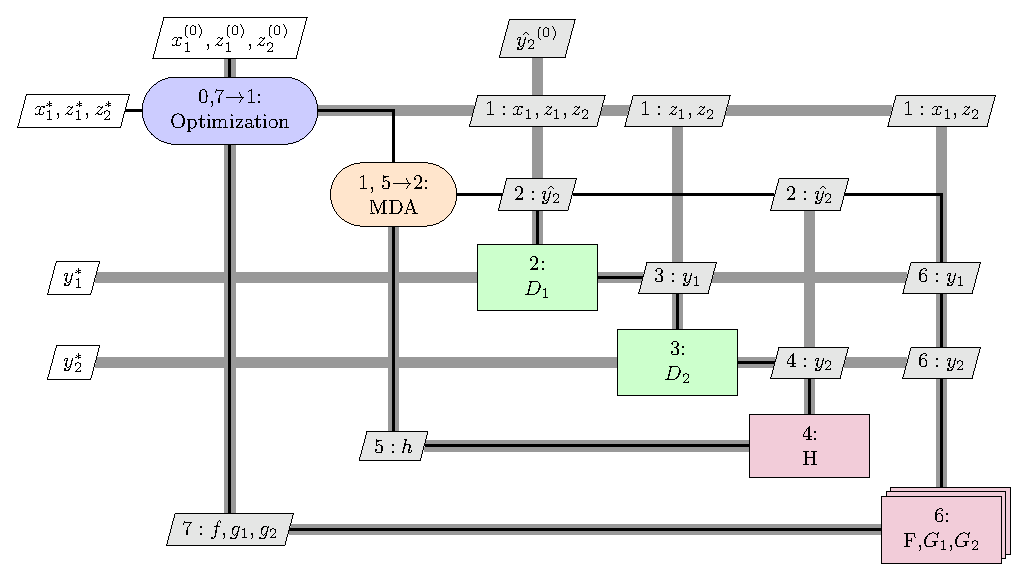
\includegraphics[height=.25\textheight]{XDSM/simple}
        \caption{XDSM for Eq. \ref{eqn:simple}, with a gauss-siedel iteration and MDF solution architecture. \label{fig:XDSM_simple}}
        \end{center}
    \end{figure}

    Although XDSM captures part of the functional aspects of FDT, it leaves out the variables themselves.  
    As a result, all variable information is aggregated 
    so that for the problem from Eq. \ref{eqn:simple_fpf} you can say that $A$ 
    depends on $B$ or vice versa, but you can't identify which 
    individual variables are interacting in the dependency cycle. 
    Without the detailed variable information, you can't construct the compatibility 
    constraints necessary to implement the problem. Additionally, XDSM 
    requires the use of solver and optimizer blocks to represent 
    the relationship between design variables and objectives/constraints. 
    By introducing solver or optimizer blocks XDSM automatically provides
    some kind of solution strategy. The XDSM for Eq. \ref{eqn:simple} is 
    given in Figure \ref{fig:XDSM_simple}. This diagram is shown with an 
    assumed gauss-siedel iteration scheme and a MDF solution architecture. 
    Hence XDSM is too specific for use with a fundamental problem formulation. 

    Of all the methods, REMS comes the closest to fully describing a problem formulation,
    but lacks the ability to represent optimziers and solvers in more specific problem 
    formulations. While XDSM does include optimizers and constraints, it relies on 
    their presence and can't be used for a more fundamental problem statement. 
    We propose a new graph syntax that combines the key features of REMS and XDSM
    and provides new language to enable more complete description of MDAO problems. 

